\documentclass[10pt]{article}
\setlength{\parskip}{0.25\baselineskip}
\usepackage[margin=1in]{geometry} 
\usepackage{amsmath,amsthm,amssymb, graphicx, multicol, array}
\usepackage[font=small,labelfont=bf]{caption}
\usepackage{tikz}
\usepackage{float}

\newcommand{\supp}{{\text{supp}}} 
\newcommand{\bv}{{\text{BV}}}
\newcommand{\ac}{{\text{AC}}}

\newenvironment{problem}[2][]{\begin{trivlist}
\item[\hskip \labelsep {\bfseries #1}\hskip \labelsep {\bfseries #2.}]}{\end{trivlist}}

\begin{document}
 
\title{Homework \#5}
\author{Eric Tao\\
Math 233: Homework \#5}
\maketitle

\begin{problem}{Question 1}

Prove that every meromorphic function on $S^2$ is rational.

\end{problem}
\begin{proof}[Solution]

Let $f$ be a meromorphic function on $S^2$. First, we consider the poles of $f$. We claim that there may only be finitely many poles.

Suppose not, that is, suppose that the set of poles of $f$, $A \subset S^2$ were at least countably infinite. Then, we may construct a sequence of points $\{a_n\}$ such that each $a_i$ is distinct. Because $S^2$ is compact then, we have that there exists a convergent subsequence. However, by definition, $A$ has no limit points, a contradiction. Thus, $A$ must be at most finite.

Now, if we restrict to $S^2 \setminus A$, where $A$ is still the poles of $f$, $f$ is holomorphic. Then, if we look at the zeros, by Theorem 10.18, we must have that there are finitely many again, for the same reason as the argument on the poles above. We may apply 10.18 because the arguments to prove that theorem do not change with the inclusion of the point and neighborhood around infinity. Since $A$ is the set of poles, i.e. $f \not = 0$ on $A$, there are only finitely many 0s on all of $S^2$.

Therefore, define the following rational function, for $a_i \in A$ the poles of $f$ with multiplicity $m_i$ and $b_i \in B$ the zeros of $f$, with multiplicity $n_i$:

$$ R(z) = \frac{\prod_{b_i \in B} (z - b_i)^{n_i}}{ \prod_{a_j \in A} (z - a_j)^{m_j}} $$

where we treat infinity specially, if we have that the point at infinity is a 0, then $\infty \in A$ and the corresponding polynomial looks like $1/z^{m_j}$ and vice versa, if the point at infinity is a pole, then $\infty \in B$ and the corresponding polynomial looks like $z^{n_i}$.

Consider $f/R$ as a function on $\mathbb{C}$. Of course, by definition, because of how we've defined $R$, to have poles with the same multiplicity as $f$ at the same points, for each $a_j$ where $f$ had a pole, $f$ has a removable singularity there. Because we have only finitely many $a_j$ also, the values that $f$ takes on at these points achieves a maximum. This argument holds as well for the zeros of $f$ against the zeros of $R$, so that this function is actually holomorphic, as the denominator then will never vanish.

Lastly, considering the behavior as $\lim_{|z| \to \infty}$, that is exactly the behavior at the point at infinity. And in the same way, $f$ and $R$ must cancel out. Thus, we have that $f/R$ must be a bounded, holomorphic function on $\mathbb{C}$, and thus constant on $\mathbb{C}$. But, by continuity, this extends onto $S^2$, and thus, $f/R$ is a constant on $S^2$. Therefore, we have that:

$$f(z) = \alpha R(z), \alpha \in \mathbb{C}$$

and thus, $f$ is rational.

\end{proof}

\begin{problem}{Question 2}

Let $\Omega = \{ z : |z| < 1 \} \cap \{ |2z - 1| > 1 \}$, and suppose $f \in \mathcal{H}(\Omega)$.

(a) Must there exist a sequence of polynomials $P_n$ such that $P_n \to f$ uniformly on compact subsets of $\Omega$?

(b) Must there exist a sequence of polynomials $P_n$ that converges to $f$ uniformly on all of $\Omega$?

(c) If we add more stipulations on (b), does the answer change? 

\end{problem}

\begin{proof}[Solution]

We start by graphing our domain $\Omega$:

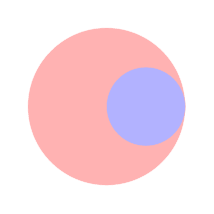
\begin{tikzpicture}
\filldraw[color=white, fill=red!30, ultra thin](0,0) circle (1);
\filldraw[color=red!30, fill=blue!30, ultra thin](0.5,0) circle(0.5);
\end{tikzpicture}

where the $x,y$ axes are identified as the real and imaginary axes. In particular, the red denotes the region $|z| < 1$ and the blue denotes the region $|2z - 1| < 1$. As such, $\Omega$ should be identified as the region that is red, but not blue. Further, it should be noted that due to a limitation of the graphing software, that although there appears to be red to the right of the blue circle, that the blue circle cannot be enclosed, since the boundaries of these circles intersect at $z = 1$.

As such, we claim that this region is simply connected. The only place where we could have issues is a loop enclosing the blue circle, and because the two circles meet at $z = 1$, there does not exist a loop in the red region that encloses the blue circle since $z=1$ is not within our region.

Thus, lifting this back into the Riemann sphere, we consider $S^2 \setminus \Omega$. In particular, we notice that this is path connected, and thus connected. It's clear that for any two points in $|z| > 1$ or any two points in $|2z - 1| < 1$, that they are path connected, so we pick one point in each region. Well, if we let $z_1 \in \{ z : |2z - 1| < 1 \}$, and $z_2 \in \{ z : |z| > 1 \}$, simply take the path $\gamma_1(t) = z_1(t) + (1-t)$, that is, the line between $z_1$ and $z = 1$, and $\gamma_2$ to be any path joining $z=1$ and $z_2$. Then, joining the two paths gives us a path from $z_1, z_2$, and thus, $S^2 \setminus \Omega$ is connected.

Then, we apply theorem 13.9. Since $S^2 \setminus \Omega$ is connected, we may take $A = \{ \infty \}$ and thus, there exists $P_n$ polynomials that converge to $f$ uniformly on comapct subsets.

(b)

Following remark 13.8, suppose not, and choose $\alpha = 1/2$, choose $K = \overline(\Omega)$, and take $f \in \mathcal{H}(\Omega)$ as:

$$ f= \frac{1}{z - 1/2}$$

Define $m = \max\{ |z - \alpha | : z \in K \}$. Since $K$ is compact, we know that this is finite. Since $P_n \to f$ uniformly on all of $\Omega$, we may choose $n$ such that $|P(z) - f(z)| < 1/m$ for all $z \in \Omega$. Then, we would have that:

$$ |P(z) - f(z)| < 1/m \implies |P(z) -\frac{1}{z - 1/2}| < 1/m \implies |(z - 1/2)P(z) - 1| < \frac{z - 1/2}{m} < 1$$

by the definition of $m$, and algebraic manipulation.

However, we notice that $K$ includes the boundary $| 2z - 1 | = 1$. Looking at the compact set $| 2 z - 1 | \leq 1$, we notice that $(z - 1/2)P(z) - 1$ is a holomorphic function on this set, being a polynomial, and thus, by the maximum modulus principle, since this is true for the boundary, it must be true as well for the interior.

Thus,  we have that at the point $z = 1/2$, that 

$$  |(z - 1/2)P(z) - 1| = |(1/2 - 1/2)P(1/2) - 1| = |-1| = 1 < 1$$

a contradiction. Thus, we may not have a sequence of polynomials necessarily for arbitrary $f \in \mathcal{H}(\Omega)$ that converge uniformly for all of $\Omega$.

(c)

If instead, $f$ were holomorphic on an open set that not only contains the closure of $\Omega$, but also contains the almost hole at $|2z - 1| < 1$, then we get (b) to be true. This would come about as a fast result of 13.9, where we take our compact set to be $K = \overline{\Omega} \cup |2z - 1 | \leq 1$. Otherwise, if we merely have an open set containing a neighborhood of $\overline{\Omega}$, we could still have issues where our new open set, $\Omega'$ may not be simply connected, and thus, we may not have a sequence of polynomials, merely rational functions, that converge uniformly on $K$.

\end{proof}

\begin{problem}{Question 3}

Is there a sequence of polynomials $P_n$ such that $P_n(0) = 1$ for all $n$, but $P_n(z) \to 0$  as $n \to \infty$?

\end{problem}

\begin{proof}[Solution]

Define the following sets:

$$ \begin{cases} K_n' = \overline{D}(0,\frac{1}{2n}) \\ K_n^{''} = \{  z : \frac{1}{n} \leq |z| \leq n, 0 \leq \text{arg}(z) \leq 2\pi - \frac{1}{n} \}  \end{cases}$$ 

That is, $K_n'$ is the closed disk centered at $0$ with radius $1/2n$, and $K_n^{''}$ is part of a annulus, with inner radius $1/n$, and outer radius $n$, stretching from $0 \leq \theta \leq 2\pi - 1/n$. It should be clear that both of these are closed and bounded sets, and thus, compact.

Define $K_n$ as $K_n' \cup K_n^{''}$. Of course, this is a compact set as well. Further, if we look at the compliment, it is connected, due to the gap in the annulus. Lastly, it should be obvious that $K_n' \supset K_{n+1}'$ and $K_n^{''} \subset K_{n+1}^{''}$. Further, $\cup_{n} K_n^{''} = \mathbb{C} \setminus \{ 0 \}$, and $\cap_n K_n' = \{ 0 \}$.

Let $U_n', U_n^{''}$ be neighborhoods on $K_n', K_n^{''}$ such that $U_n' \cap U_n^{''} = \emptyset$.

$$f_n(z) = \begin{cases} 1 & \text{ if } z \in U_n' \\ 0 & \text{ if } z \in U_n^{''} \end{cases} $$

Of course, because this is constant on disconnected regions, this is holomorphic on $U_n = U_n' \cap U_n^{''}$, since constants are differentiable.

Then, by Theorem 13.7, there exists a polynomial $P_n$ defined on $U_n$ such that $| P_n(z) - f_n(z) | < 1/n$ for all $z \in K_n$.

Consider this collection of polynomials $P_n$. Since polynomials are entire, these are defined on all of $\mathbb{C}$. 

For the point $z = 0$, we may see that $\lim_{n \to \infty} P_n(0) = 0$, since if we let $\epsilon > 0$ be given, then we may just choose $N$ such that $\frac{1}{N} < \epsilon$. By our definition of $P_n$ then, we have that for all $n > N$, we have that:

$$| P_n(z) - f_n(z) | < 1/n$$, defined on $K_n'$. However, $0 \in K_n'$ for each $K_n'$, so we have that for all $n > N$:

$$| P_n(0) - 1 | = | P_n(0) - f_n(0) | < \frac{1}{n} < \frac{1}{N} < \epsilon$$

Now, instead, let $z \in \mathbb{C} \setminus \{ 0 \}$. Let $\epsilon > 0$ be given. Let $r = |z|, \theta = \text{arg}(z)$. There exists an $R$ such that $r \in (1/R, R)$ since $1/n \to 0, n \to \infty$. There exists a $\Theta$ such that $\theta \in (0,2\pi - 1/\Theta)$ modulo $2\pi$, since $2\pi - 1/n \to 2\pi$. There exists an $N$ such that $\frac{1}{N} < \epsilon$.

Choose $M = \min(N, R, \Theta)$.

Then, $z \in K_m^{''}$ for each $m \geq M$, and by construction, and the same argument used for $z = 0$:

$$ | P_n(z) - 0 | =  | P_n(z) - f_n(z) | < \frac{1}{n} < \frac{1}{N} < \epsilon$$

and we are done.

\begin{center}
\includegraphics[width=\linewidth]{partial_annulus}
\end{center}

Where this is for $n=2$, $K_2'$ is the red disk, and $K_2^{''}$ is the region between the blue and green disks.

\end{proof}

\begin{problem}{Question 4}

Is there a sequence of polynomials $P_n$ such that:

$$\lim_{n\to\infty} P_n(z) = \begin{cases} 1 & \text{  if } \Im(z) > 0 \\ 0 &  \text{  if } \Im(z) = 0  \\ -1 & \text{  if } \Im(z) < 0 \end{cases} $$ 

where $\Im(z)$ denotes the imaginary part of $z$.

\end{problem}
 
\begin{proof}[Solution]

Define the following sets:

$$\begin{cases} A_n = \{ z :  -n \leq \Re(z) \leq n, \frac{1}{n} \leq \Im(z) \leq n \} \\ B_n = \{ z :   -n \leq \Re(z) \leq n, -\frac{1}{2n} \leq \Im(z) \leq \frac{1}{2n} \} \\ C_n = \{  z :  -n \leq \Re(z) \leq n, -n \leq \Im(z) \leq -\frac{1}{n} \}\end{cases}$$

It should be clear that $A_n, B_n, C_n$ are closed, bounded, and thus compact. Further, we should see that $A_n \subset A_{n+1}, B_n \subset B_{n+1}, C_n \subset C_{n+1}$, $\cup_n A_n =   H^+, \cup_n B_n = \{ z : \Im(z) = 0 \}, \cup_n C_n  = H^-$, where $H^+, H^-$ denote the upper half and lower half plane, respectively.

In the same way in Question 3, we define $K_n = A_n \cup B_n \cup C_n$. This is still a compact set, where the complement is connected, and we can take neighborhoods of $A_n, B_n, C_n$ to find a open set that contains our compact set, with one component per compact component. (One example is something like:

$$ \begin{cases}U_n =  \{ z : -n - 1 < \Re(z) < n+1, \frac{1}{1.5n} < \Im(z) < 2n \} \\ U_n' =   \{ z :   -n-1 < \Re(z) < n+1, -\frac{1}{1.75n} < \Im(z) < \frac{1}{1.75n} \} \\ U_n^{''} =  \{  z :  -n-1 < \Re(z) < n +1, -n-1 < \Im(z) < -\frac{1}{1.5n} \} \end{cases} $$

Then, we may define on these neighborhoods:

$$f_n(z) = \begin{cases} 1 & \text{ if } z \in U_n \\  0 & \text{ if } z \in U_n' \\ -1 & \text{ if } z \in U_n{''} \end{cases}$$

Of course, since $f_n(z)$ is constant on components, it is holomorphic on each component, and thus holomorphic on the entire open set.

Then, by Theorem 13.7, we may find a polynomial $P_n$ such that $| P_n(z) - f_n(z) | < 1/n$ for all $z \in K_n$. 

In the same way as question 3, if $\Im(z)  = 0$, then there exists an $N$ such that $|\Re(z)| < N$. Let $\epsilon > 0$ be given, and choose $L$ such that $1/L < \epsilon$. Choose $M = \max(L,N)$. Since $M > | \Re(z)|$, we have that $z \in B_n$. Thus, we apply the estimate, for any $m > M$:

$$ |P_m(x) - 0 | = |P_m(x) - f_m(x) | < \frac{1}{M} \leq \frac{1}{L} < \epsilon $$

The same goes for $\Im(z) \not = 0$, we just find $L$ large enough that $z \in A_l$ or $z \in C_l$, and $M$ such that $1/M < \epsilon$. Then, pick $N$ to be the max, and if $\Im(z) > 0$ we look on $A_n$, else we look in $C_n$, and we get that:

$$ | P_n(z) - 1 | = | P_n(z) - f_n(z) | < \epsilon $$ for $z \in H^+$ and the same idea for $-1$ on $H^-$.

Picture:

\begin{center}
\includegraphics[width=\linewidth]{partial_boxes}
\end{center}

where this is $n = 2$, $A_2$ in green, $B_n$ in blue, and $C_n$ in purple.

\end{proof}
  

\begin{problem}{Question 5}

Find necessary and sufficient conditions on $a,b,c,d \in \mathbb{C}$ such that the linear fractional transformation 

$$T: z \to \frac{az + b}{cz + d}$$

maps the upper half plane onto itself.

\end{problem}

\begin{proof}[Solution]

First, consider the case $c = 0$. In such a case, we can write our transformation as:

$$ z \to \frac{a}{d} z + \frac{b}{d}$$

For this to map objects from the upper half plane into the upper half plane, we notice that $\frac{a}{d}$ must be strictly real. Otherwise, we could express $\frac{a}{d} = re^{i\theta}$ for $\theta \not = 0$, and choose $\varphi \in (0,\pi)$ such that $\varphi + \theta \in [\pi, 2\pi]$ modulo $2\pi$. Then, any point along the portion of the line $e^{i \varphi}$ contained in the upper half plane would be mapped outside.

Furthermore, $\frac{a}{d}$ must be strictly positive. If not, then we notice that for any choice of $b, d$, so long as we choose $\Im(z) > |\frac{1}{d}\Im(b)|$, that:

$$\Im\left(\frac{a}{d} z + \frac{b}{d}\right) = \frac{a}{d} \Im(z) + \frac{1}{d} \Im(b) < 0$$

So, WLOG, we may choose $a, d \in \mathbb{R}^+$, as any other choice would just be scaled by a constant factor $\alpha$. Now, we look at $\frac{b}{d}$. We notice that here too, if $d \in \mathbb{R}$, then so must $b$. Suppose not. Then, we could express $b = x + yi, y \not = 0$. If $y < 0$, then choose $z$ such that for $z = w + vi$, $av < |y|$, which we can do because for a fixed $|y|, a$, the Archimidean principle guarantees us a positive real number between 0 and this quantity. Then, looking at the imaginary portion of our transformation, we would have that:

$$\Im\left(\frac{a}{d} z + \frac{b}{d}\right) = \frac{a}{d} \Im(z) + \frac{1}{d} \Im(b) = \frac{1}{d}(av + y)  < 0$$

and thus we land outside of our upper half plane. Conversely, if $y > 0$, then we notice that with the imaginary part above, that:

$$\Im\left(\frac{a}{d} z + \frac{b}{d}\right) = \frac{a}{d} \Im(z) + \frac{1}{d} \Im(b) = \frac{1}{d}(av + y)   > \frac{y}{d}$$

Thus, for any $z$ in the upper half plane with imaginary portion in $(0,\frac{y}{d})$ there cannot exist a $z'$ such that $z' \to z$.

Therefore, $y = 0$, and thus if $a,d$ are real and positive, then $b$ must also be real.

Now, these are necessary, but are they sufficient? Let $a,b,d \in \mathbb{R}$ such that $\frac{a}{d} > 0$. Well, this should be clear. Let $z'$ be a point in the upper half plane. Then, we wish to find $z$ such that:

$$ \frac{a}{d}z + \frac{b}{d} = z' $$

Rewrite $z' = u + vi$. Then, we have that:

$$ \frac{a}{d} z = \left(u - \frac{b}{d}\right) + vi \implies z = \left(\frac{du}{a}  - \frac{b}{a}\right) + \frac{dv}{a} i $$

We see that since $\frac{d}{a} > 0, v > 0$ because $z'$ in the upper half plane, and our hypothesis, then $\frac{dv}{a} > 0$. Thus, $z$ lies in the upper half plane, and $z'$ has a preimage. In parallel with the next section, we will rewrite this as taking $ad > 0$, as $\frac{d}{a} > 0 \iff ad > 0$.

Now, suppose $c \not = 0$.

Well, again, we look for necessary conditions first. We know that such a transformation must take the reals to the reals, since they are the boundary of the upper half plane. Thus, we have that, for $x \in \mathbb{R}$, that:

$$ \frac{ax  + b }{cx + d} = \frac{(ax + b) (\overline{cx + d})}{ |cx + d|^2 } = \frac{a\overline{c} x^2 + x(b\overline{c} + a \overline{d}) + b\overline{d} }{ | cx + d|^2} \in \mathbb{R}$$

where we denote the complex conjugate by the line overhead. Well, since the denominator is real, we only have to look to check that the numerator is real as well. In particular, since this holds for all $x \in \mathbb{R}$, this implies that each coefficient must independently be real. Thus, we have the conditions:

$$ \begin{cases} a\overline{c} \in \mathbb{R} \\ b\overline{c} + a \overline{d} \in \mathbb{R} \\ b \overline{d} \in \mathbb{R} \end{cases} $$

For this to be true, then, we must have that, for real parameters $r_a, r_b, r_c, r_d$, that, from equations 1, 3, we have that:

$$ a = r_a e^{i \theta}, c = r_c e^{i\theta}, b = r_b e^{i \varphi} d = r_d e^{i \varphi} $$

Substituting into equation 2 then, we see that:

$$  b\overline{c} + a \overline{d} = r_b r_c e^{i(\varphi - \theta)} + r_a r_d e^{i(\theta - \varphi)} $$

Looking at only the imaginary part, we see that we need the following quantity to vanish:

$$ r_b r_c \sin(\varphi - \theta) + r_a r_d \sin(\theta - \varphi) = r_b r_c \sin(\varphi - \theta) - r_a r_d \sin(\varphi - \theta) = \sin(\varphi - \theta)(r_b r_c - r_a r_d)  = 0$$

We notice that if $(r_b r_c - r_a r_d) = 0$, then we land in the degenerate case where $ad - bc = 0$ due to our definitions of $a,b,c,d$ earlier. Thus, to satisfy this equation, we would need that

$$  \sin(\varphi - \theta)  = 0 \iff \varphi - \theta = \pi n \implies \varphi = \theta \text{ or } \varphi = \theta + \pi $$

modulo $2\pi$ of course. This implies we have two cases, either $\varphi = \theta$ and thus $a,b,c,d \in \mathbb{R}$, as we can always divide through by our complex angle, or $\varphi = \theta + \pi$ and thus dividing through by $e^{i \theta}$, we are left with $e^{i \pi} = -1$ for $b,d$. Regardless then, up to a complex coefficient, we can say that $a,b,c,d \in \mathbb{R}$. 

Now, looking back at that conjugate equation, but armed with taking $a,b,c,d \in \mathbb{R}$, and looking at $z \in H^+$ instead of $x \in \mathbb{R}$, we see that:

$$  \frac{az  + b }{cz + d} =  \frac{(az + b) (\overline{cz + d})}{ |cz + d|^2 } = \frac{ac|z|^2 + adz + bc\overline{z} + bc}{ |cz + d|^2} $$

For this to land back in $H^+$, we must have that the imaginary component is positive. In particular, then, if $z = x + yi, y > 0$, we must have that:

$$ \Im\left( \frac{ac|z|^2 + adz + bc\overline{z} + bc}{ |cz + d|^2} \right) = \frac{1}{|cz + d|^2} (ady - bcy) = \frac{y}{|cz + d|^2} (ad - bc) > 0 \implies ad - bc > 0 $$

So now, we need only prove that this is a sufficient condition. We show that $T$ admits an inverse, injective. Let $z \in H^+$, and consider the transformation:

$$S: z \to \frac{dz - b}{-cz + a} $$

In particular, we can see that:

$$T(S(z)) = T\left(\frac{dz - b}{-cz + a}\right) = \frac{a\left(\frac{dz - b}{-cz + a}\right) + b}{c\left(\frac{dz - b}{-cz + a}\right) +d } = \frac{ adz - ba + ba - bcz }{cdz - bc + ad - cdz} = \frac{z(ad - bc)}{ad - bc} = z$$

and

$$ S(T(z)) = S\left( \frac{az  + b }{cz + d}\right) =   \frac{d\left( \frac{az  + b }{cz + d}\right) - b}{-c\left( \frac{az  + b }{cz + d}\right) + a} = \frac{daz + db - bcz - bd}{-acz -bc + acz + ad} = \frac{z(ad - bc)}{ad - bc} = z$$

Further, since $ad - bc \not = 0$, we see that for $S$, that implies that $da - (-b)(-c) = ad - bc \not = 0$, so that $S$ is also injective. Thus, $T$ is injective, and admits an inverse on $H^+$, and thus must be bijective, therefore onto. 
\end{proof}

\end{document}